%%%%%%%%%%%%%%%%%%%%%%%%%%%%%%%%%%%%%%%%%%%%%%%%%%%%%%%%%%%%%%%%%%%%%%%%%%%%%
% 26/05/2010
% edited by Bill Lampos
%
% Feel free to use (copy) the structure (latex formatting source code)
% but not the content of this document.
%
%%%%%%%%%%%%%%%%%%%%%%%%%%%%%%%%%%%%%%%%%%%%%%%%%%%%%%%%%%%%%%%%%%%%%%%%%%%%%
\documentclass[compress,red]{beamer}
\usepackage{etex}
\mode<presentation>
%Warsaw, Antibes, Berlin
\usetheme{Warsaw}
% other themes: AnnArbor, Antibes, Bergen, Berkeley, Berlin, Boadilla, boxes, CambridgeUS, Copenhagen, Darmstadt, default, Dresden, Frankfurt, Goettingen,
% Hannover, Ilmenau, JuanLesPins, Luebeck, Madrid, Maloe, Marburg, Montpellier, PaloAlto, Pittsburg, Rochester, Singapore, Szeged, classic

\usecolortheme{default}
% color themes: albatross, beaver, beetle, crane, default, dolphin, dov, fly, lily, orchid, rose, seagull, seahorse, sidebartab, structure, whale, wolverine

%\usefonttheme{serif}
% font themes: default, professionalfonts, serif, structurebold, structureitalicserif, structuresmallcapsserif

% pdf is displayed in full screen mode automatically
\hypersetup{pdfpagemode=FullScreen}

% define your own colours:
\definecolor{c}{rgb}{1,0,0}
\definecolor{Blue}{rgb}{0,0,1}
\definecolor{Green}{rgb}{0,1,0}
\definecolor{magenta}{rgb}{1,0,.6}
\definecolor{lightblue}{rgb}{0,.5,1}
\definecolor{lightpurple}{rgb}{.6,.4,1}
\definecolor{gold}{rgb}{.6,.5,0}
\definecolor{orange}{rgb}{1,0.4,0}
\definecolor{hotpink}{rgb}{1,0,0.5}
\definecolor{newcolor2}{rgb}{.5,.3,.5}
\definecolor{newcolor}{rgb}{0,.3,1}
\definecolor{newcolor3}{rgb}{.80,.25,.33}
\definecolor{darkgreen1}{rgb}{0, .35, 0}
\definecolor{darkgreen}{rgb}{0, .6, 0}
\definecolor{darkred}{rgb}{.75,0,0}

\xdefinecolor{olive}{cmyk}{0.64,0,0.95,0.4}
\xdefinecolor{purpleish}{cmyk}{0.75,0.75,0,0}

\newcommand{\tab}[1]{\hspace{.065\textwidth}\rlap{#1}}

% \usepackage{beamerinnertheme_______}
% inner themes include circles, default, inmargin, rectangles, rounded

%\usepackage{beamerouterthemesmoothbars}
% outer themes include default, infolines, miniframes, shadow, sidebar, smoothbars, smoothtree, split, tree

\useoutertheme[subsection=false]{smoothbars}

% to have the same footer on all slides
%\setbeamertemplate{footline}[text line]{xxx xxx xxx}
%\setbeamertemplate{footline}[text line]{} % or empty footer
\setbeamercolor{footlinecolor}{fg=white,bg=darkred}
\renewcommand\footnoterule{{\color{black}\hrule height 0.1pt width \paperwidth}}

\makeatother
\setbeamertemplate{footline}{%
  \leavevmode%
\textcolor{white}{\hrule}
  \footnoterule
  \hbox{%
  \begin{beamercolorbox}[wd=\paperwidth,ht=0.10in,dp=0.5ex,center]{footlinecolor}
    \hfill{} \inserttitle\hfill\insertsubtitle\hfill
	\insertframenumber{}/\inserttotalframenumber    \vskip0pt plus.5fill
  \end{beamercolorbox}}%
  \vskip0pt%
}
\makeatletter
%\setbeamertemplate{navigation symbols}{}

% include packages
\usepackage[T1]{fontenc}
\usepackage[utf8]{inputenc}
\usepackage{subfig}
\usepackage{multicol}
\usepackage{amsmath}
\usepackage{animate}
\usepackage{epsfig}
\usepackage{graphicx}
\usepackage[all,knot]{xy}
\usepackage[font=small,labelfont=bf]{caption}
\xyoption{arc}
\usepackage{url}
\usepackage[export]{adjustbox}
\usepackage{multimedia}
\usepackage{hyperref}
\usepackage{setspace}

\title{Onion Routing in Predictable \\ Delay Tolerant Networks}
\author{Adrián Antúnez Veas}
\institute{dEIC, Universidad Autónoma de Barcelona}
\date{\scriptsize Julio, 2015}

\begin{document}\thispagestyle{empty}
\AtBeginSection[]
{
%  \begin{frame}
%    \frametitle{Table of Contents}
%    \tableofcontents[currentsection,
%  sectionstyle=show/shaded,
%  subsectionstyle=show/show/hide]
%  \end{frame}
}

\frame{
	\titlepage
}

\section[Index]{}
\frame{\tableofcontents[hideallsubsections]
}

\section{Background}
\subsection{DTN overview}
\begin{frame}
\frametitle{DTNs overview}
\begin{block}{Definition}
Delay and disruption tolerant networks.
\end{block}
\bigskip 
Based on the \alert{\emph{store-carry-and-forward}} principle.\\
\bigskip
\begin{block}{Some applications...}
\begin{itemize}
\item Lacking continuous connectivity.
\item Long or variable delays.
\item Achieve independent network.
\end{itemize}
\end{block}
\end{frame}

\subsection{Onion routing}
\begin{frame}
\frametitle{Onion routing overview}
Source \textit{S} wants to send an anonymous message to \textit{C} (destination).
\bigskip
\begin{block}{Onion routing phases}
\begin{enumerate}
\item \textit{S} chooses a path $p=(S),A,B,C$ from source to destination.
\item \textit{S} encrypts the message with the pre-shared key of \textit{C}, \textit{B} and \textit{A}.
\item \textit{S} sends the message.
\end{enumerate}
\end{block}
\bigskip
\centering 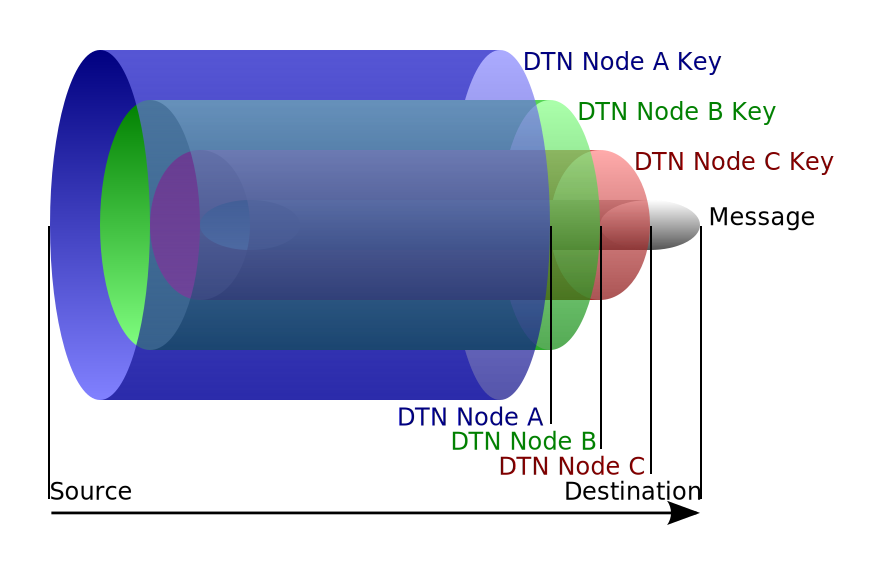
\includegraphics[width=.5\linewidth]{../paper/imgs/onion}
%Each intermediate node, decrypts the message with his private key revealing the next encryption layer. At the end, the destination gets the fully decrypted message.
%Comment that the key management process will be done in a early step.
\end{frame}

\subsection{Oracle schemes}
\begin{frame}
\frametitle{Oracle schemes overview}
\begin{block}{Definition}
Oracle schemes have knowledge of the network and its evolution.
\end{block}
\bigskip
\begin{block}{Contacts oracle}
Contacts oracle can answer any contact related question between two nodes in any point in time.
\end{block}
\bigskip
\begin{block}{Predictable (deterministic) DTNs}
Networks where the behaviour is known in advance or where a repetitive action occurs over time.
\end{block}
\end{frame}

\section{Motivation and objectives}
\subsection{Motivation and objectives}
\begin{frame}
\frametitle{Motivation and objectives}
\begin{block}{Main objective}
Achieve anonymous communications over an independent network.
\end{block}
\bigskip
\begin{block}{Onion routing along with predictable DTNs}
\begin{itemize}
\item Find a way to \alert{represent the contacts} of the network.
\item Find a method to perform the previous \alert{path selection} step.
\item \alert{Security analysis} of our proposal.
\item Show how this method performs in a \alert{real scenario}.
\end{itemize}
\end{block}
\end{frame}

\section{Proposal}
\subsection{Contact representation}
\begin{frame}
\frametitle{Contact representation}
\begin{block}{Structure used}
A dynamic graph $G = (V,E)$ as a way of contact representation.
\end{block}
\bigskip
\begin{itemize}
\item \textit{G:} Dynamic graph representing the evolution of the network.
\item \textit{V:} Each \alert{node} of the network is represented by \alert{vertices}.
\item \textit{E:} Each \alert{contact} between nodes is represented by \alert{edges}.
\end{itemize}
\bigskip
\begin{block}{Each edge will have two attributes}
\begin{itemize}
\item Instant of time when the contact began.
\item  Duration of the contact.
\end{itemize}
\end{block}
\end{frame}

\subsection{Dynamic graph example}
\begin{frame}
\frametitle{Dynamic graph example}

\only<1>{
\begin{figure}
\addtocounter{subfigure}{0}
\subfloat[Complete graph]{
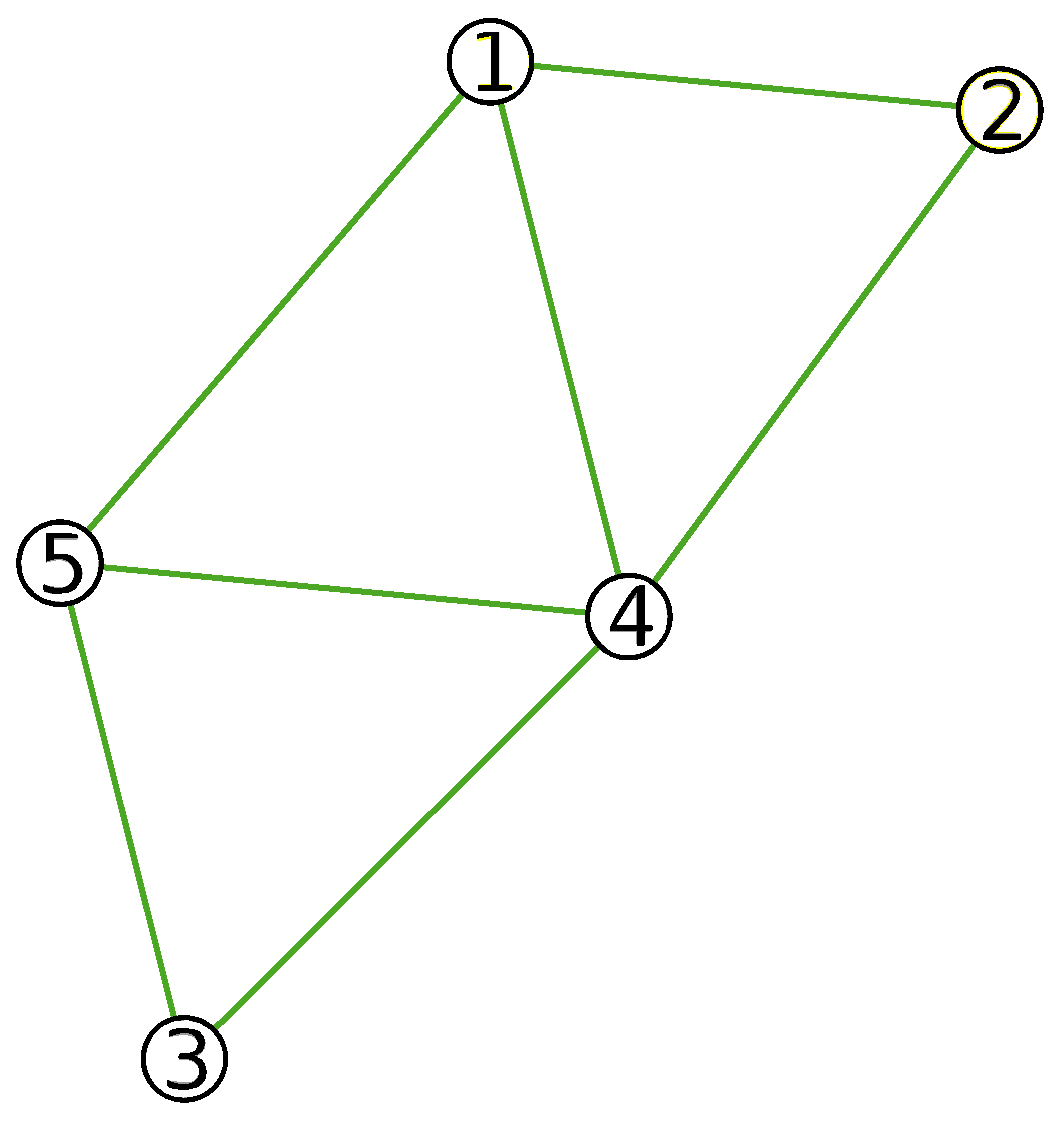
\includegraphics[width=0.4\textwidth]{../paper/imgs/example-dynamic/full}}
\subfloat[t=0]{
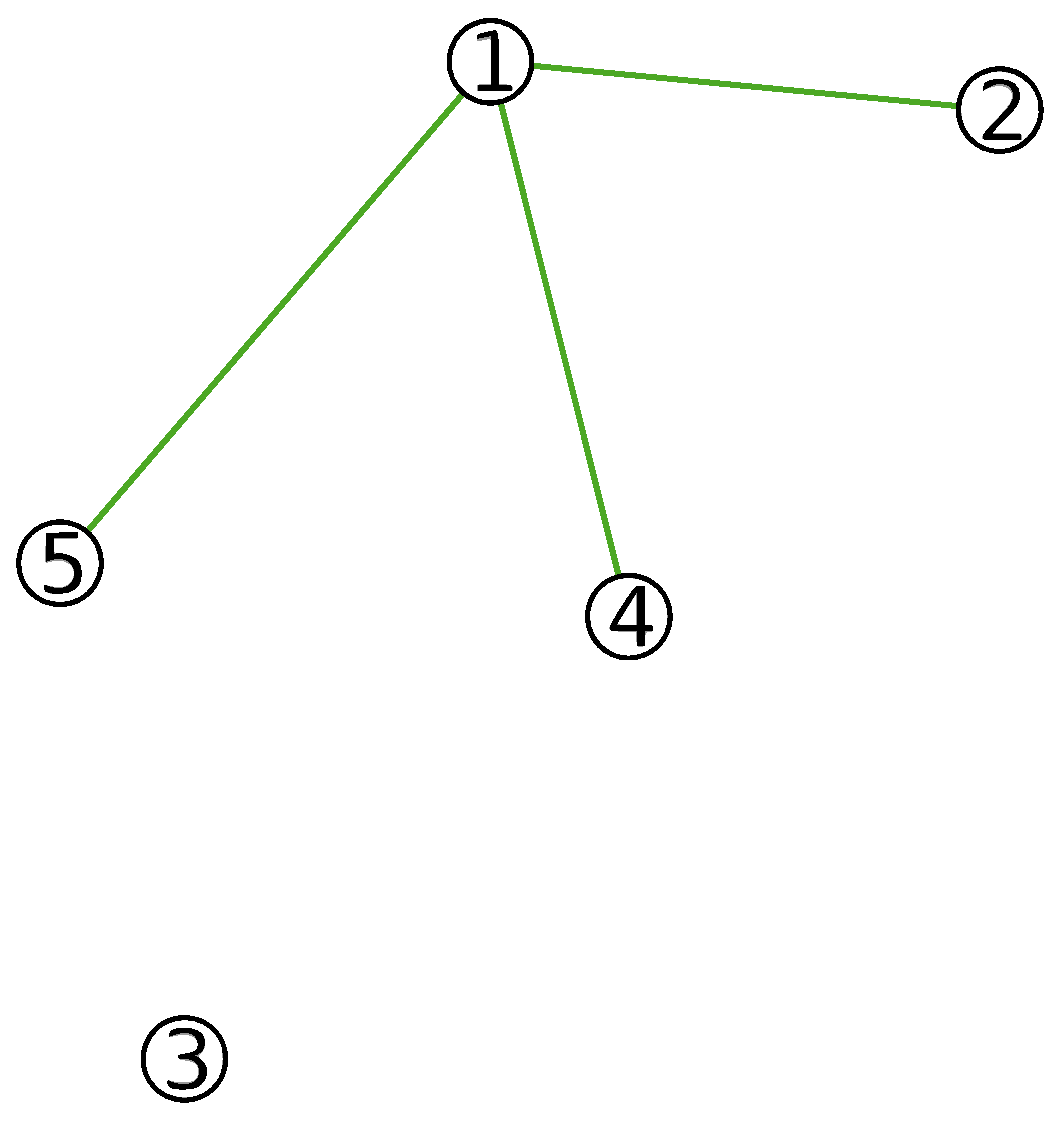
\includegraphics[width=0.4\textwidth]{../paper/imgs/example-dynamic/t0}}
\end{figure}
}
\only<2>{
\begin{figure}
\addtocounter{subfigure}{-2}
\subfloat[Complete graph]{
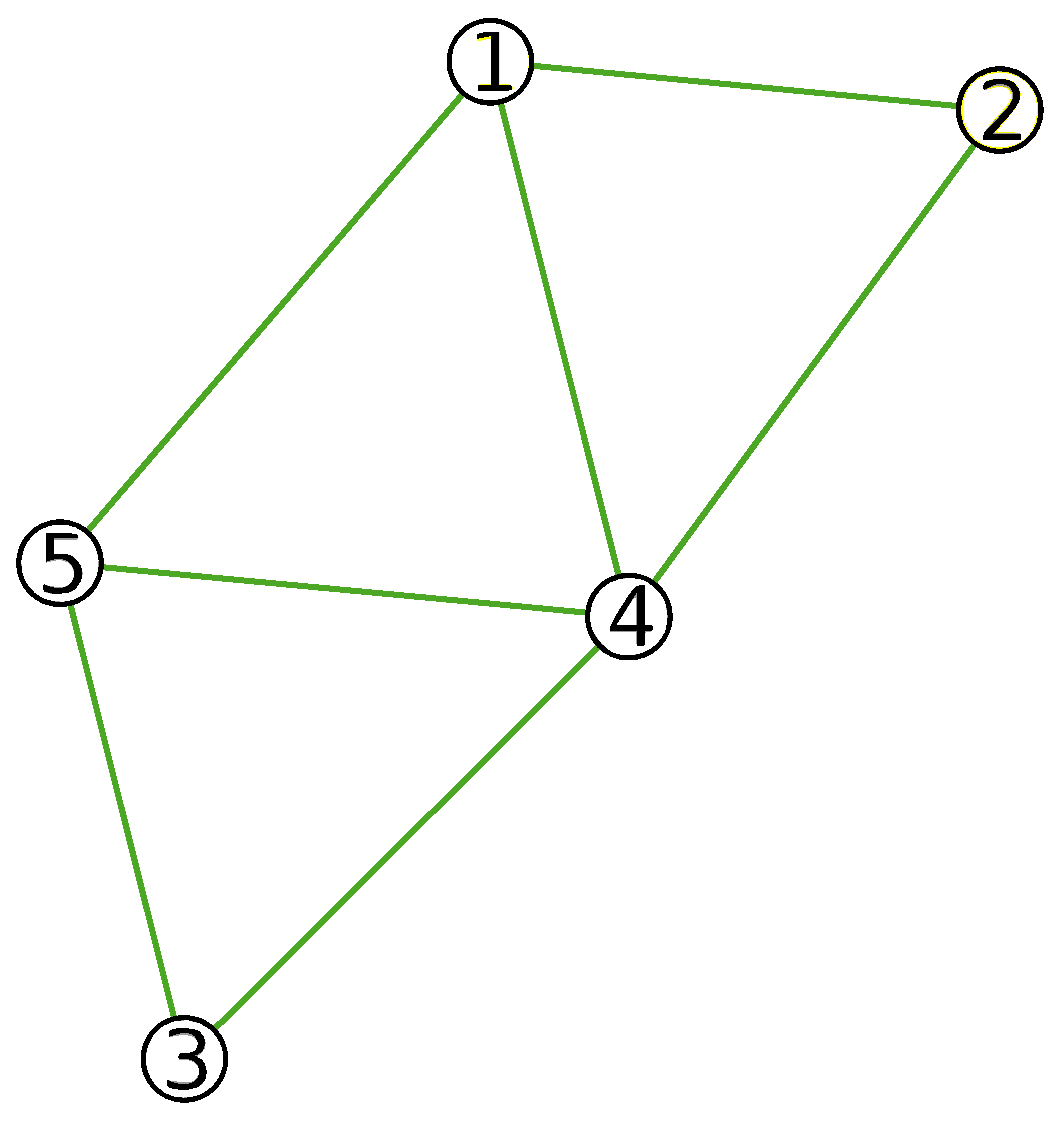
\includegraphics[width=0.4\textwidth]{../paper/imgs/example-dynamic/full}}
\addtocounter{subfigure}{1}
\subfloat[t=1]{
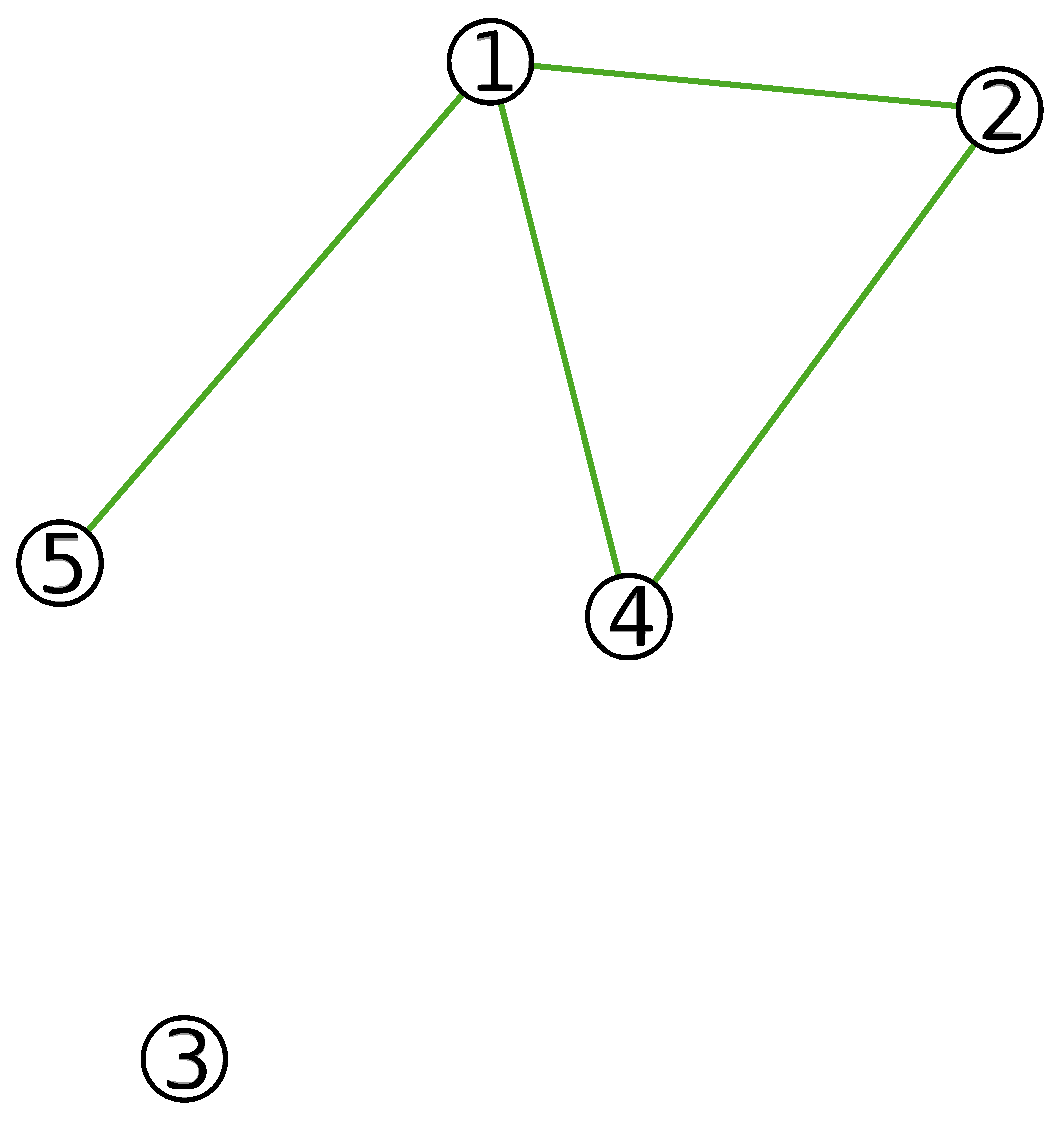
\includegraphics[width=0.4\textwidth]{../paper/imgs/example-dynamic/t1}}
\end{figure}
}
\only<3>{
\begin{figure}
\addtocounter{subfigure}{-3}
\subfloat[Complete graph]{
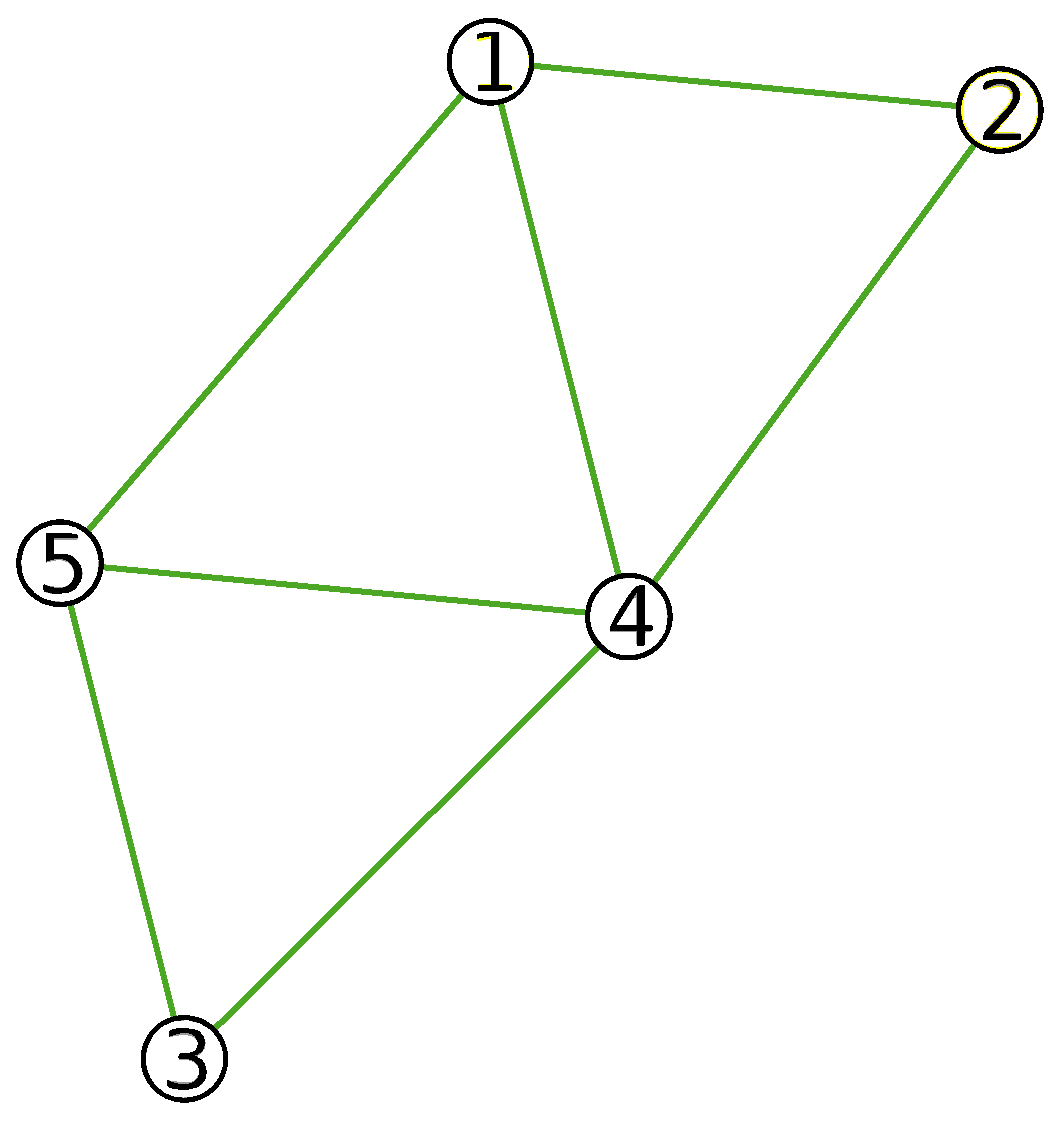
\includegraphics[width=0.4\textwidth]{../paper/imgs/example-dynamic/full}}
\addtocounter{subfigure}{2}
\subfloat[t=2]{
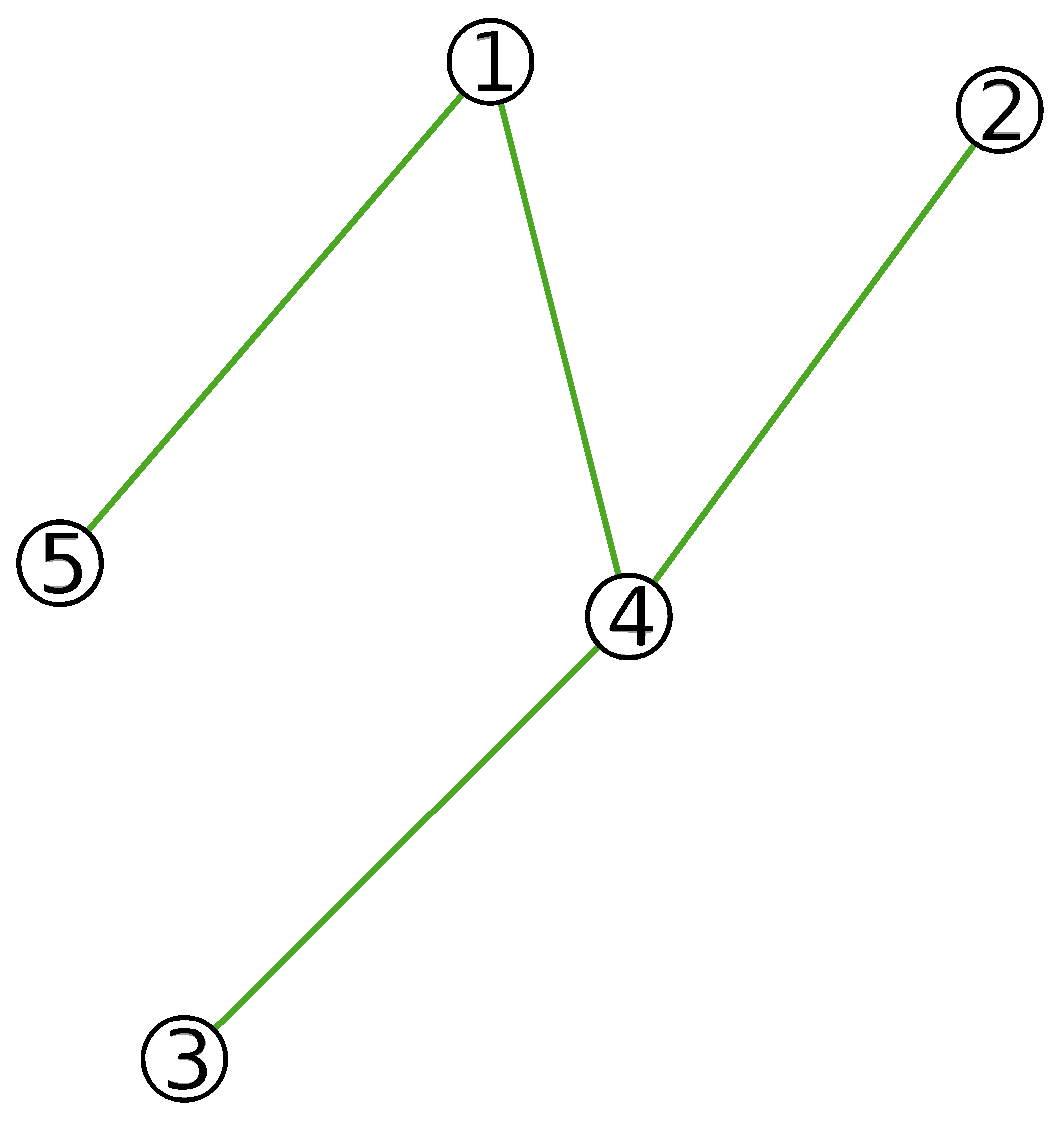
\includegraphics[width=0.4\textwidth]{../paper/imgs/example-dynamic/t2}}
\end{figure}
}
\only<4>{
\addtocounter{subfigure}{-4}
\begin{figure}
\subfloat[Complete graph]{
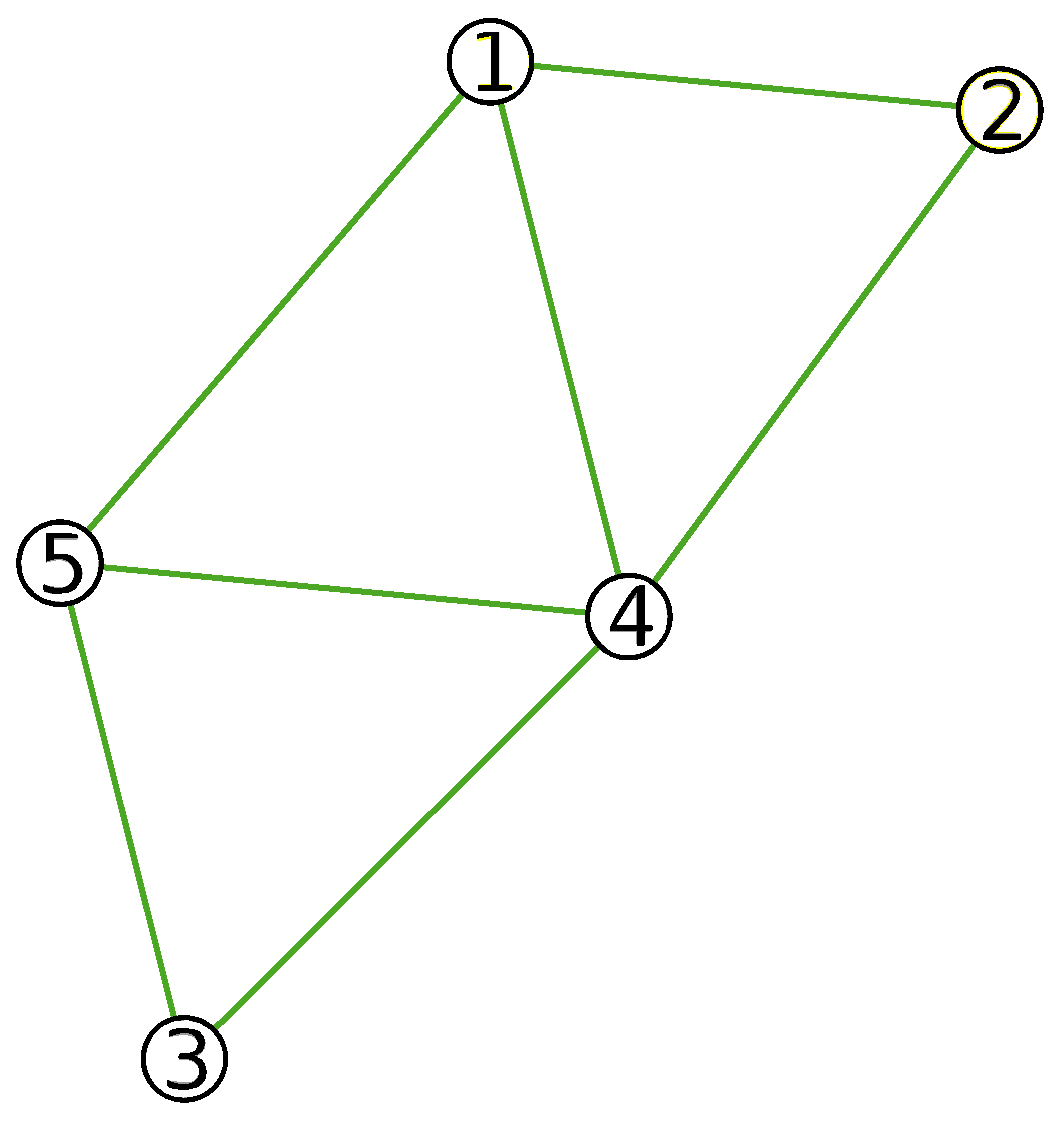
\includegraphics[width=0.4\textwidth]{../paper/imgs/example-dynamic/full}}
\addtocounter{subfigure}{3}
\subfloat[t=3]{
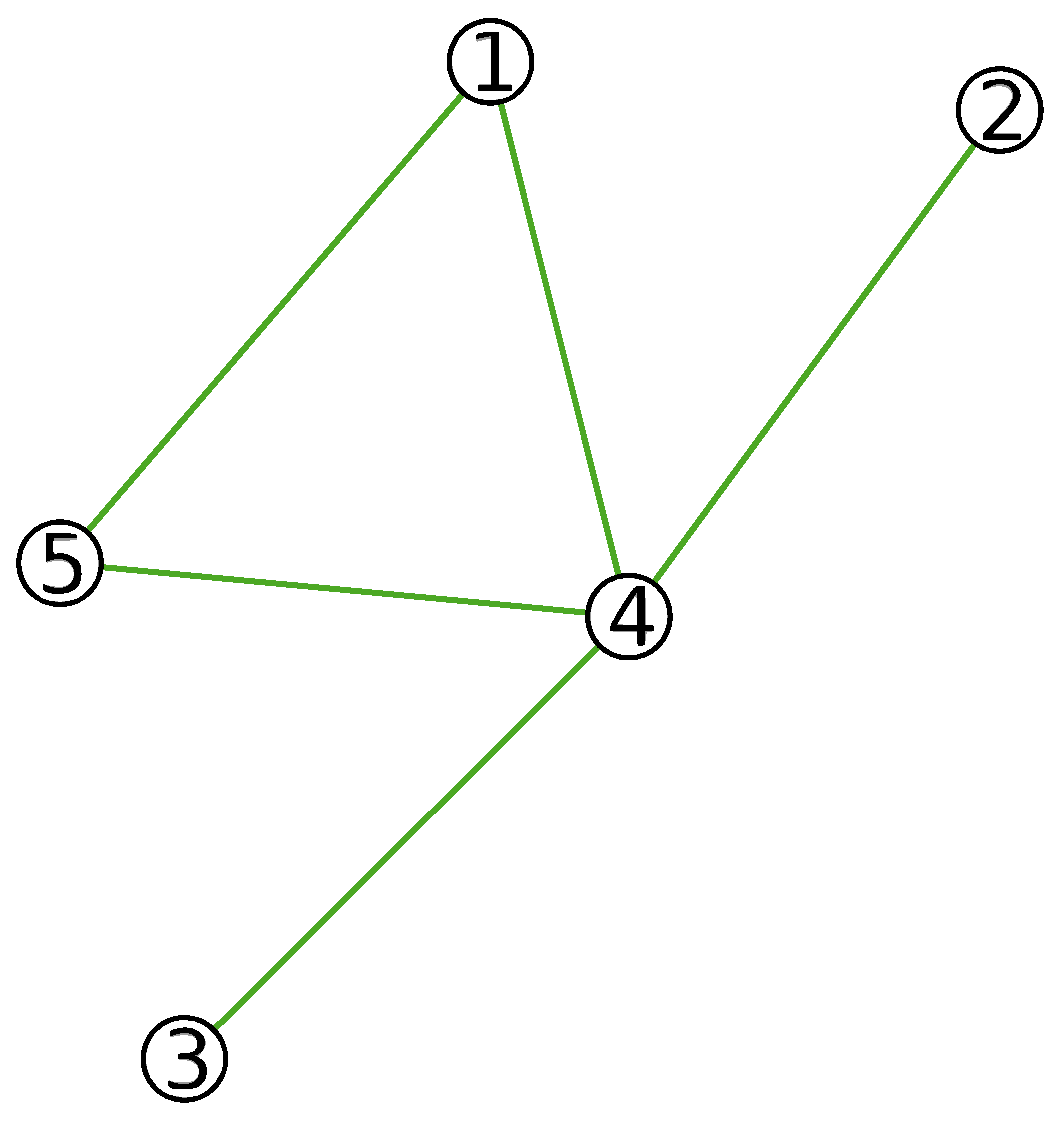
\includegraphics[width=0.4\textwidth]{../paper/imgs/example-dynamic/t3}}
\end{figure}
}
\only<5>{
\begin{figure}
\addtocounter{subfigure}{-5}
\subfloat[Complete graph]{
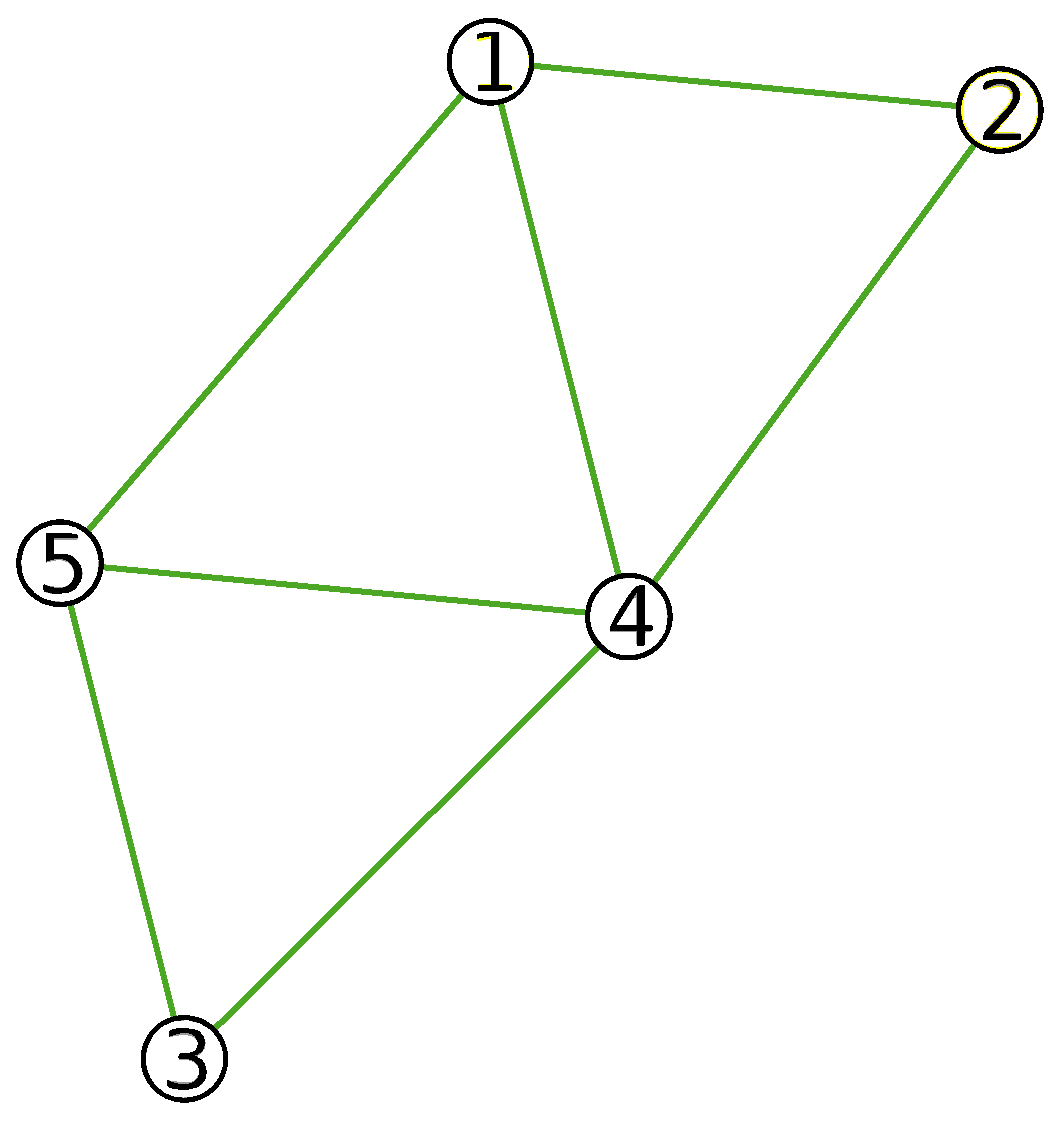
\includegraphics[width=0.4\textwidth]{../paper/imgs/example-dynamic/full}}
\addtocounter{subfigure}{4}
\subfloat[t=4]{
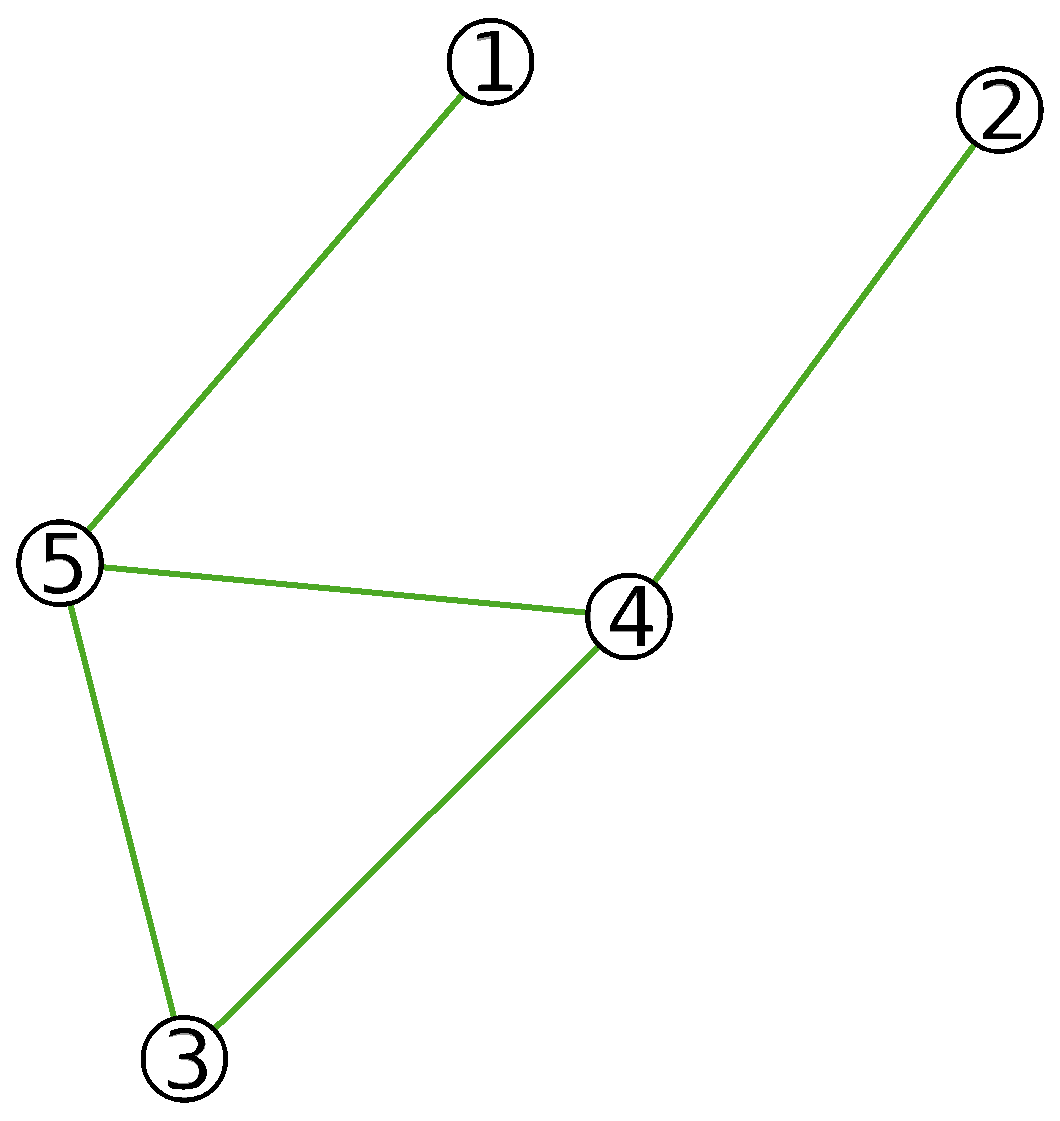
\includegraphics[width=0.4\textwidth]{../paper/imgs/example-dynamic/t4}}
\end{figure}
}
\only<6>{
\begin{figure}
\addtocounter{subfigure}{-6}
\subfloat[Complete graph]{
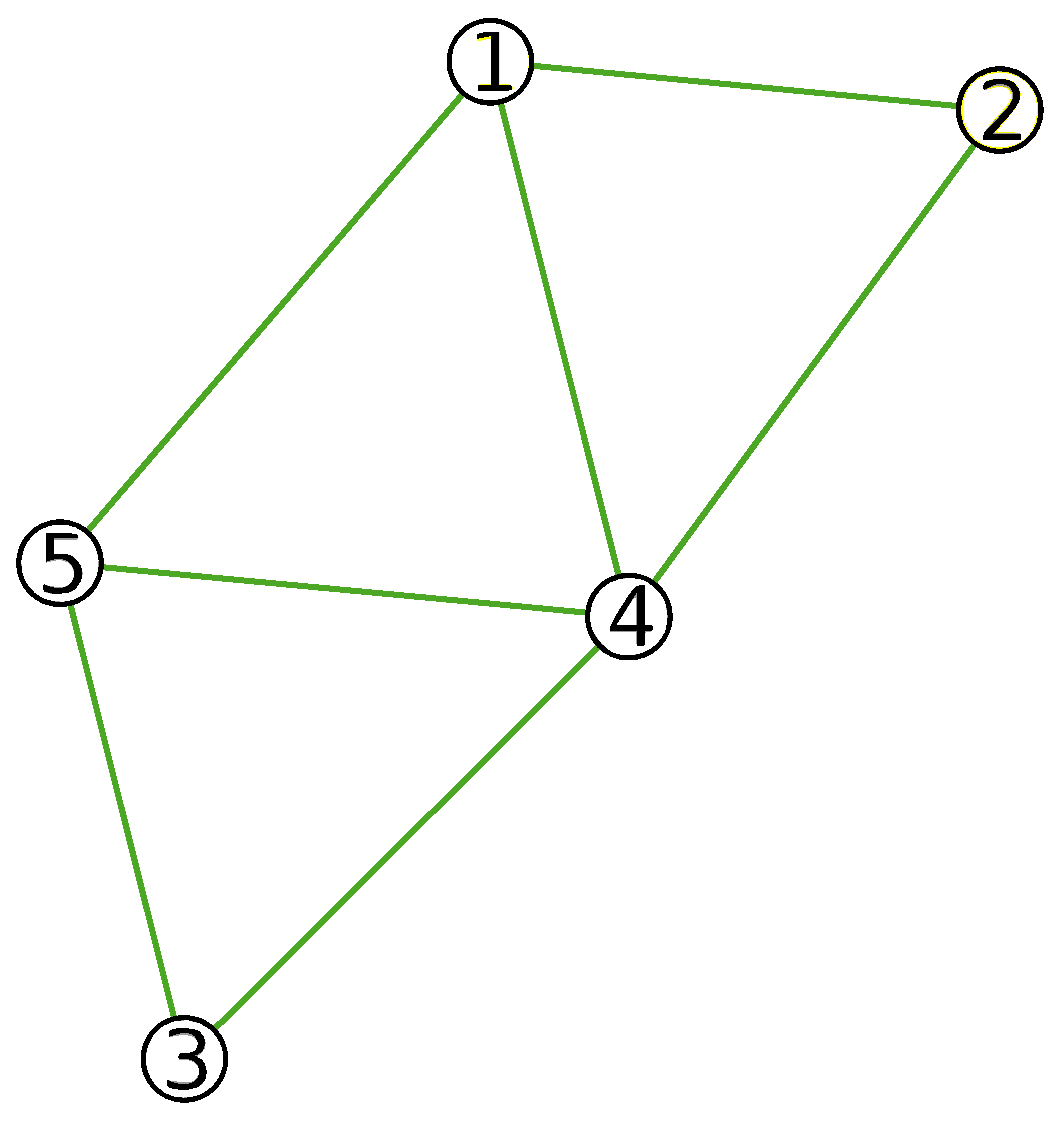
\includegraphics[width=0.4\textwidth]{../paper/imgs/example-dynamic/full}}
\addtocounter{subfigure}{5}
\subfloat[t=5]{
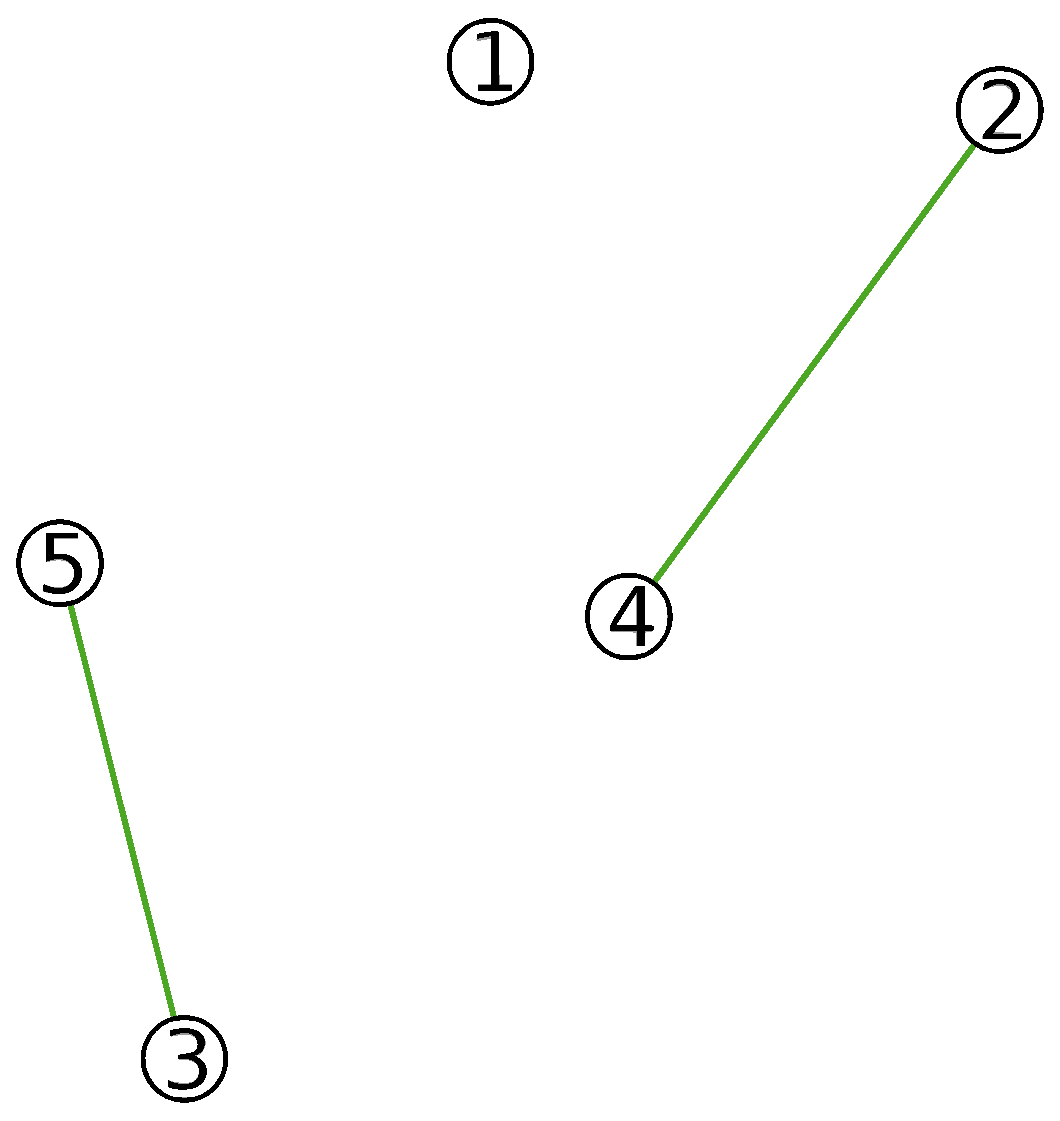
\includegraphics[width=0.4\textwidth]{../paper/imgs/example-dynamic/t5}}
\end{figure}
}
\only<7>{
\addtocounter{subfigure}{-7}
\begin{figure}
\subfloat[Complete graph]{
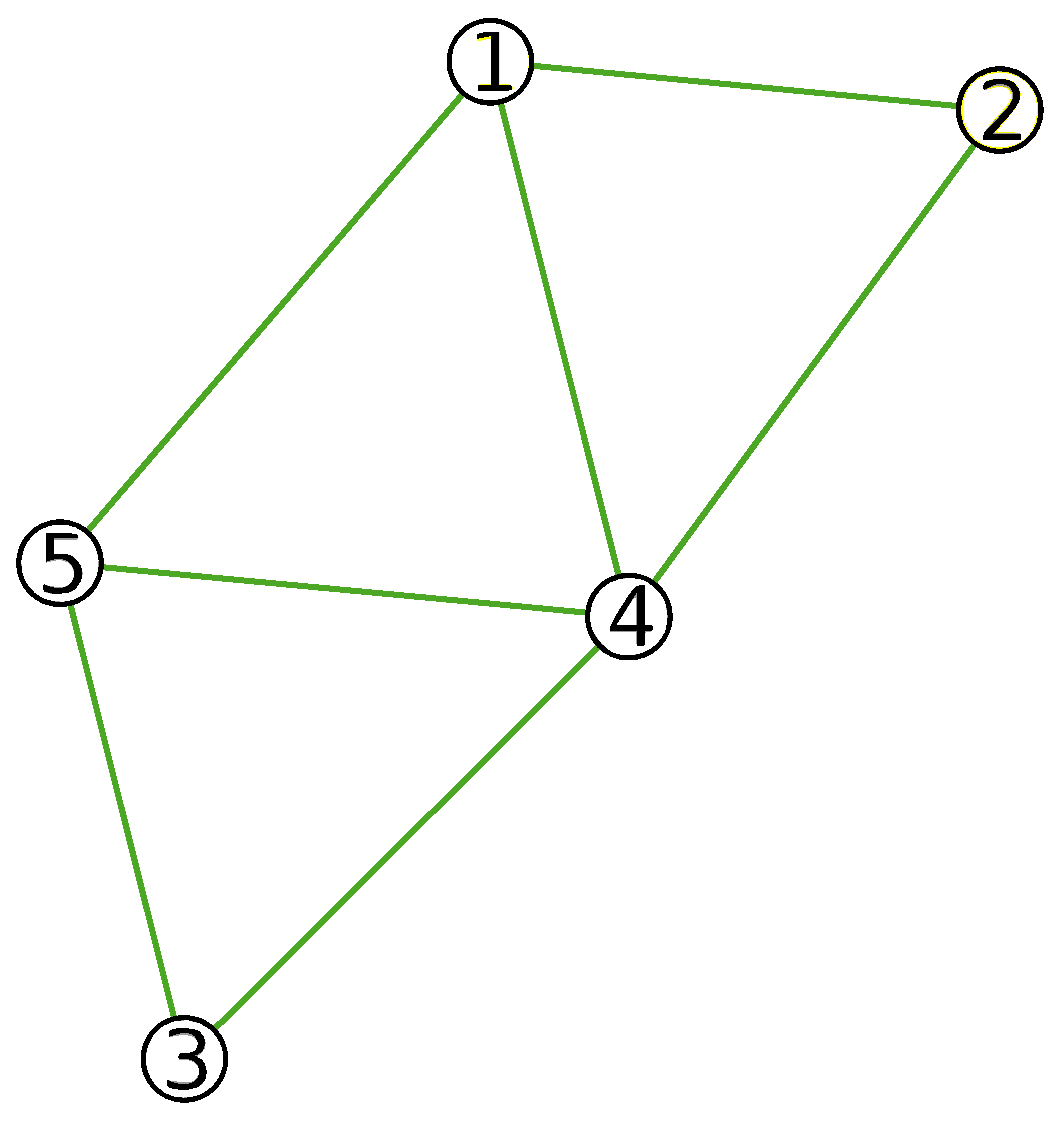
\includegraphics[width=0.4\textwidth]{../paper/imgs/example-dynamic/full}}
\addtocounter{subfigure}{6}
\subfloat[t=6]{
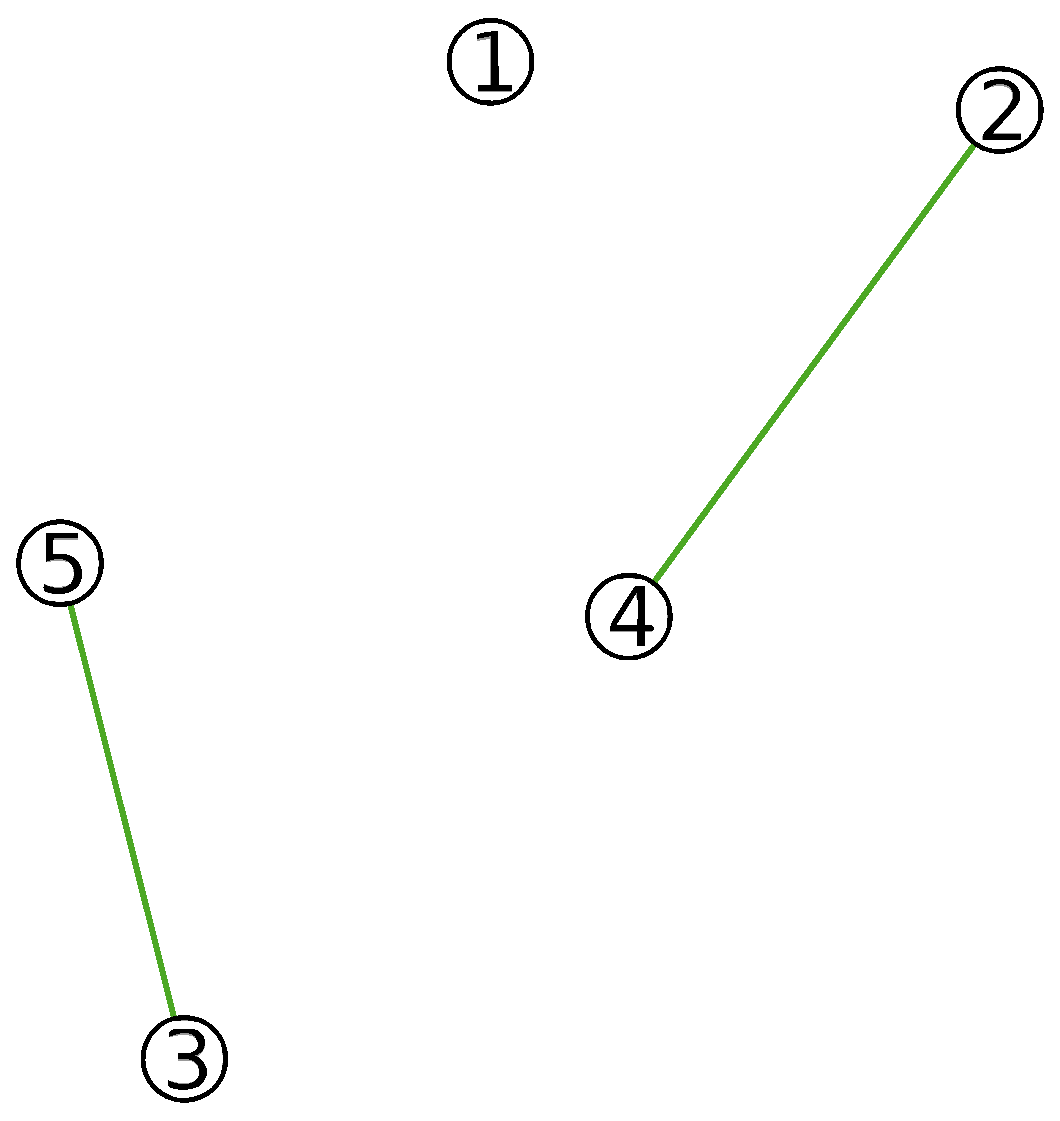
\includegraphics[width=0.4\textwidth]{../paper/imgs/example-dynamic/t6}}
\end{figure}
}
\only<8>{
\begin{figure}
\addtocounter{subfigure}{-8}
\subfloat[Complete graph]{
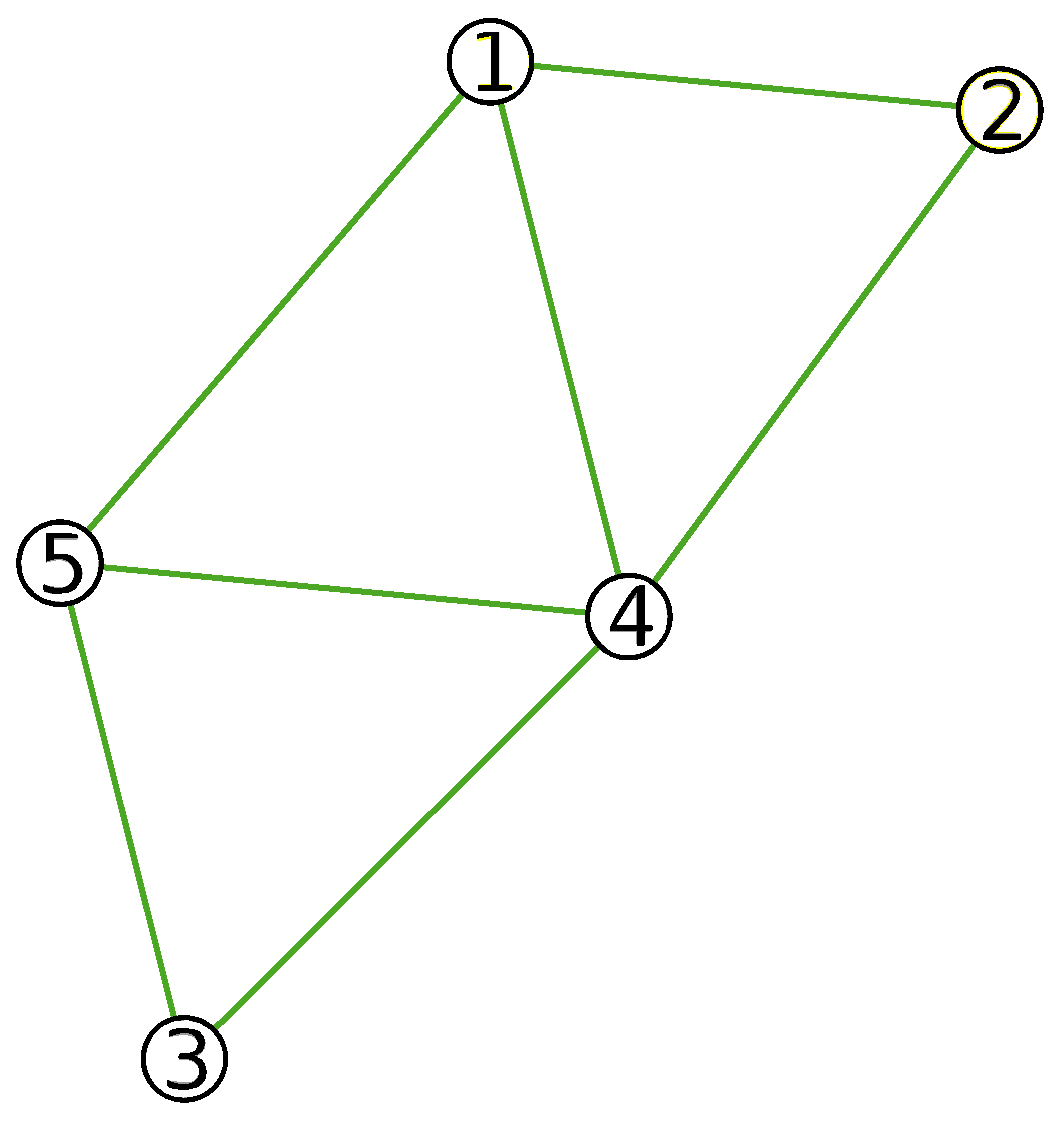
\includegraphics[width=0.4\textwidth]{../paper/imgs/example-dynamic/full}}
\addtocounter{subfigure}{7}
\subfloat[t=7]{
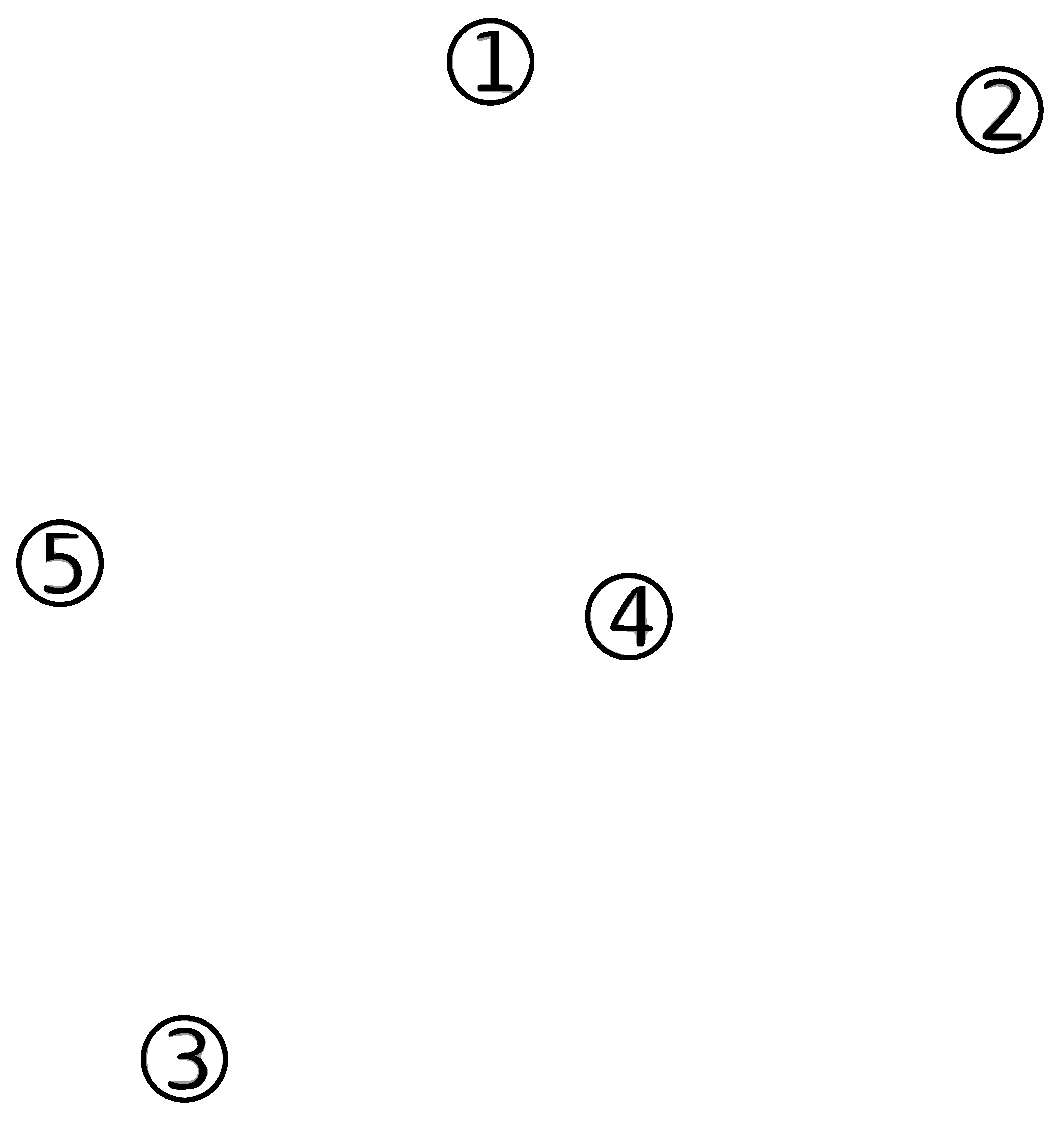
\includegraphics[width=0.4\textwidth]{../paper/imgs/example-dynamic/t7}}
\end{figure}
}
\end{frame}

\subsection{Path selection}
\begin{frame}
\frametitle{Path selection}
\begin{block}{The necessity}
In onion routing a path to perform the layering process is needed.
\end{block}
\bigskip
\begin{block}{The method}
A deterministic method \textit{f(s, d, t, n, k, tt)} is defined.
\begin{itemize}
\item \textit{s}: Source node.
\item \textit{d}: Destination node.
\item \textit{t}: Time when the message is sent.
\item \textit{n}: Number of nodes in each path.
\item \textit{k}: Maximum number of paths to be returned.
\item \textit{tt}: Transmission time.
\end{itemize}
\end{block}
\end{frame} %By this way we solve the challenging routing problem in DTNs.

\section{Security Analysis}
\subsection{Security Analysis}
\begin{frame}
\frametitle{Security Analysis}
\begin{block}{Goal}
Reveal who sent the message (uncover the source).
\end{block}
\begin{block}{Attack types}
Can be divided in two groups:
\begin{itemize}
\item Active: Actions against nodes or message modifications.
\item Passive: Just observing user traffic patterns from nodes.
\end{itemize}
\end{block}
\bigskip
\begin{block}{Active attacks}
\begin{itemize}
\item Denial of Service (DoS) attacks to neighbour nodes.
\item Message modifications.
\item Masquerading (nodes pretending to be others).
\end{itemize}
\end{block}
\end{frame}

\subsection{Passive adversaries}
\begin{frame}
\frametitle{Passive attacks}
\begin{block}{Passive attacks}
\begin{itemize}
\item Learn from the content of the message.
\item Sending node periodicity analysis.
\item Set of compromised nodes working together.
\end{itemize}
\end{block}
%{\setbeamercolor{block body}{bg=white}
\begin{block}{Example}
\begin{itemize}
\item Node 1 sent an anonymous message to node 4.
\item Node 1 message's contains a timestamp.
\item Nodes 2 and 4 have been compromised.
\item Node 5 never has sent or has forwarded a message yet.
\end{itemize}
\centering 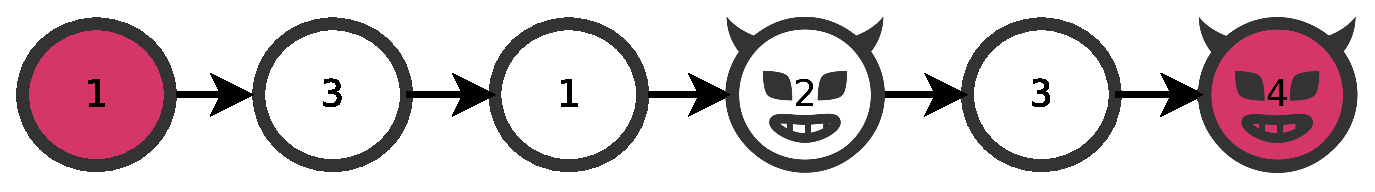
\includegraphics[width=.7\linewidth]{../paper/imgs/presentation/evil-path}
\end{block}
%}
\end{frame}

\section{Evaluation}
\subsection{NS-3 simulation scenario}
\begin{frame}
\frametitle{NS-3 simulation scenario}
\begin{block}{NS-3 definition}
NS-3 is a discrete-event simulator targeted primarily for research.
\end{block}
\bigskip
\begin{block}{Implementation details}
\begin{itemize}
\item Implemented neighbour discovery on the application layer.
\item The app polls every second to find new contact opportunities.
\item If contact is missing for 2 seconds, contact has been lost.
\end{itemize}
\end{block}
\bigskip
\end{frame}

\subsection{Mobility model}
\begin{frame}
\frametitle{Mobility model}
\begin{block}{UAB campus buses}
\begin{itemize}
\item Very small public transportation network (5 buses).
\item Every single bus makes the same route daily (deterministic).
\item Each bus 802.11b Wi-Fi hotspot with a range up to 100m.
\end{itemize}
\end{block}
\begin{figure}
\includegraphics[width=0.95\textwidth]{../paper/imgs/presentation/process}
\end{figure}
\end{frame}

\subsection{Simulation results}
\begin{frame}
\frametitle{Simulation results}
\begin{figure}
\centering 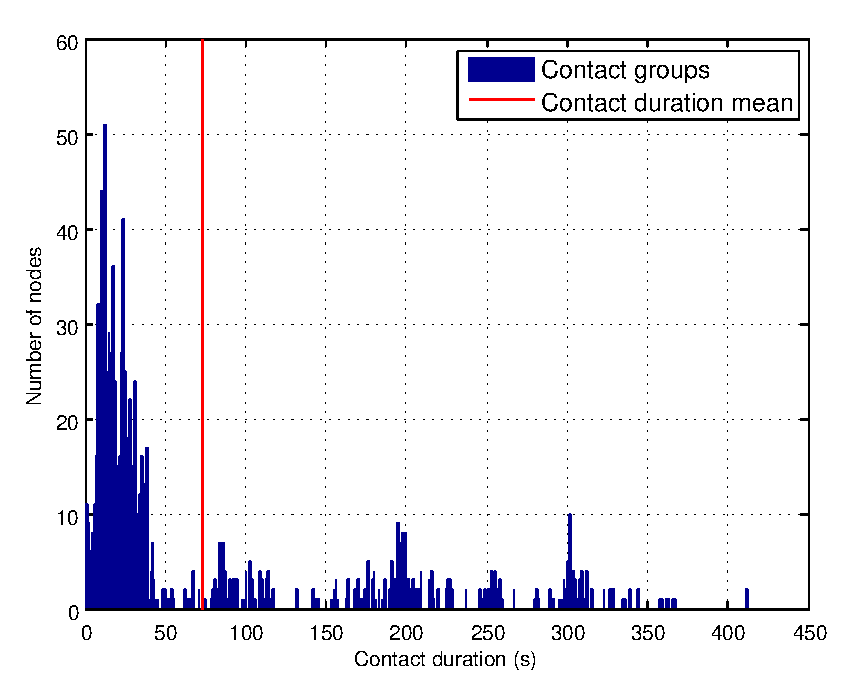
\includegraphics[width=.7\linewidth]{../paper/imgs/statistics/contacts-duration}
\caption{Contacts duration.}
\end{figure}
\end{frame}

\subsection{Simulation results (II)}
\begin{frame}
\frametitle{Simulation results (II)}
\begin{figure}
\centering 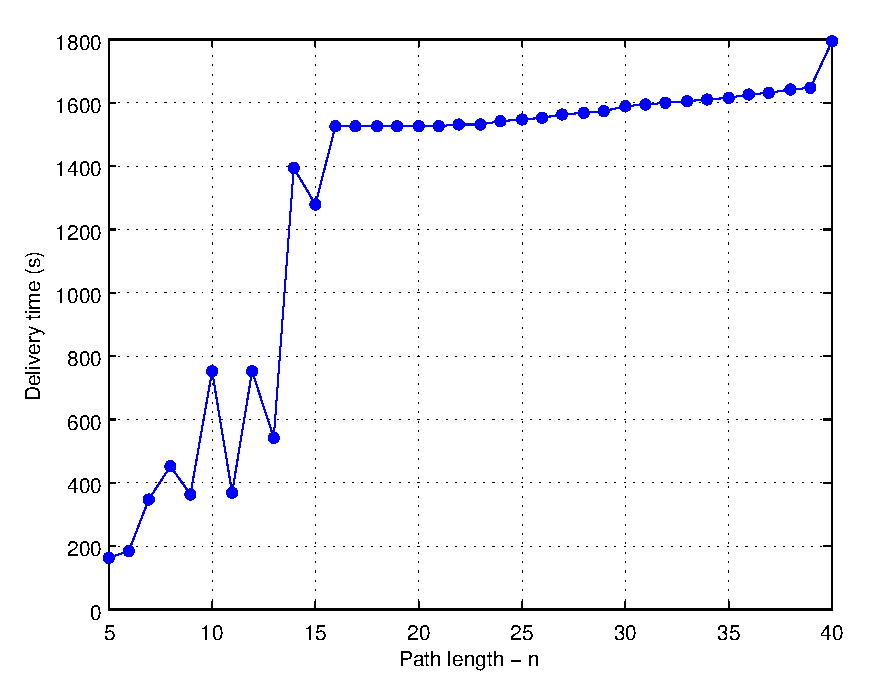
\includegraphics[width=.7\linewidth]{../paper/imgs/statistics/ntime-data}
\caption{Average delivery time considering the variation of the path length (k=10 was fixed).}
\end{figure}
\end{frame}

\subsection{Simulation results (III)}
\begin{frame}
\frametitle{Simulation results (III)}
\begin{figure}
\centering 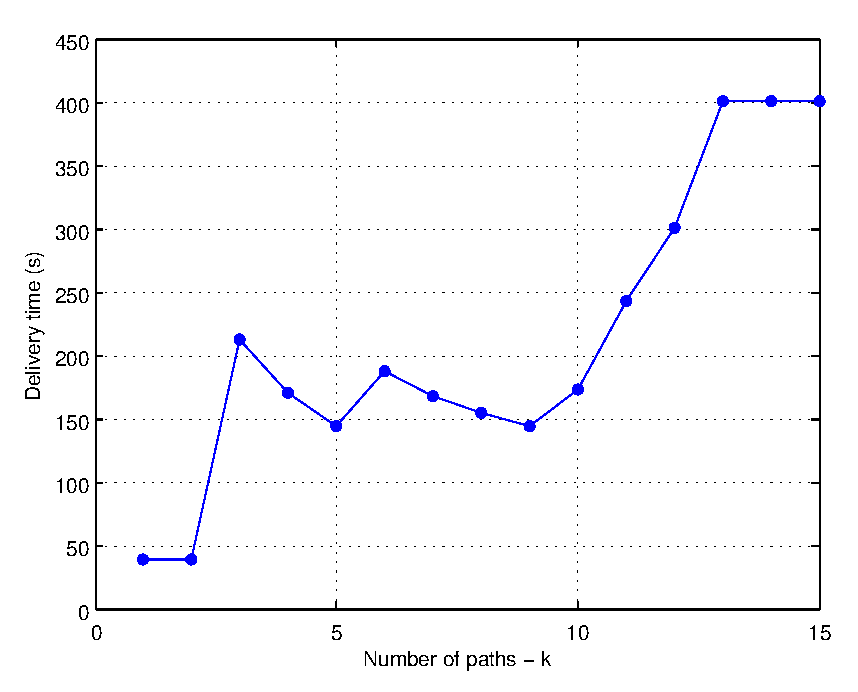
\includegraphics[width=.7\linewidth]{../paper/imgs/statistics/ktime-data}
\caption{Average delivery time considering the variation of the number of paths (n=5 was fixed).}
\end{figure}
\end{frame}

\section{Conclusions}
\begin{frame}
\frametitle{Conclusions}
\begin{block}{Conclusions}
\begin{itemize}
\item We proposed a method to use onion routing in DTNs.
\item In DTNs not always the shortest paths are the quickest ones.
\item In our method, new paths selection are not correlated to time.
\end{itemize}
\end{block}
\bigskip
\begin{block}{Future work}
\begin{itemize}
\item Search and analyse efficient ways of path selection.
\item Decrease the number of attacks using reputation systems.
\item Adapt contact representation to consider traffic modifications. %Adaptament dinàmic diari de la informació recollida
\end{itemize}
\end{block}
\end{frame}

\end{document} 